\documentclass[aspectratio=169]{beamer}

\newcommand{\const}{\texttt{\bfseries const}}

\usepackage{fontspec}
\usepackage{listings}
\usepackage{tikz}

\usetikzlibrary{arrows}
\usetikzlibrary{calc}
\usetikzlibrary{decorations.pathreplacing}
\usetikzlibrary{fit}
\usetikzlibrary{matrix}
\usetikzlibrary{positioning}
\usetikzlibrary{tikzmark}
\usetikzmarklibrary{listings}

\definecolor{solarizedRed}{RGB}{220, 50, 47}
\definecolor{solarizedBlue}{RGB}{38, 139, 210}
\definecolor{solarizedGreen}{RGB}{133, 153, 0}
\definecolor{solarizedPurple}{RGB}{108, 113, 196}

\setbeamercolor{title}{fg=solarizedBlue}
\setbeamercolor{frametitle}{fg=solarizedBlue}
\setbeamercolor{structure}{fg=solarizedBlue}

\setbeamertemplate{navigation symbols}{}
\setbeamertemplate{headline}{}
\setbeamertemplate{footline}{}
\setbeamertemplate{itemize items}[circle]
%\setbeamertemplate{footline}[frame number]

\setbeamertemplate{footline}{
  \begin{tikzpicture}[remember picture,
                      overlay,
                      shift={(current page.south west)}]
    \node [black!50, inner sep=2mm, anchor=south east]
          at (current page.south east) {\large \insertframenumber};
  \end{tikzpicture}
}

\setsansfont{Overpass}[Scale=MatchLowercase]
\setmonofont{Overpass Mono}[Scale=MatchLowercase]

\lstset{
  basicstyle=\ttfamily,
  language=C,
  escapeinside={(*@}{@*)},
  commentstyle={\color{black!35}},
}

\title{Operating System Interfaces}
\date{April 3, 2019}
\author{Jon Eyolfson}

\setbeamertemplate{title page}
{
  \begin{tikzpicture}[remember picture,
                      overlay,
                      shift={(current page.south west)}]
    \node (title) [inner sep=0, scale=2, align=left]
          at (\paperwidth / 2, \paperheight * 2 / 3)
          {\bfseries \usebeamerfont{title}\usebeamercolor[fg]{title}CS 111\\
           \usebeamerfont{title}\usebeamercolor[fg]{title}\inserttitle};
    \node (author) [scale=1.5] at (\paperwidth / 2, \paperheight / 3)
          {\insertauthor};
    \node [anchor=south west, inner sep=2mm] (cc-logo) at (0, 0)
          {
\includegraphics[scale=0.2]{cc.logo.eps}};
    \node [node distance=0, right=of cc-logo, xshift=-0.5em, yshift=-0.45em]
          {BY-SA 4.0};
    \node [anchor=south east, inner sep=2mm] at (\paperwidth, 0)
          {\texttt{1.1.0}};
    \node [anchor=south, inner sep=2mm] at ($(\paperwidth / 2, 0)$)
          {\insertdate};
  \end{tikzpicture}
}

\begin{document}

  \begin{frame}[plain]
    \titlepage
  \end{frame}

  \setcounter{framenumber}{0}

  \begin{frame}
    \frametitle{You Wouldn't Write in Binary, Would You?}

    \texttt{%
      0x7F 0x45 0x4C 0x46 0x02 0x01 0x01 0x03 0x00 0x00 0x00 0x00 0x00 0x00 0x00
      0x00 0x02 0x00 0x3E 0x00 0x01 0x00 0x00 0x00 0x78 0x00 0x01 0x00 0x00 0x00
      0x00 0x00 0x40 0x00 0x00 0x00 0x00 0x00 0x00 0x00 0x00 0x00 0x00 0x00 0x00
      0x00 0x00 0x00 0x00 0x00 0x00 0x00 0x40 0x00 0x38 0x00 0x01 0x00 0x40 0x00
      0x00 0x00 0x00 0x00 0x01 0x00 0x00 0x00 0x05 0x00 0x00 0x00 0x00 0x00 0x00
      0x00 0x00 0x00 0x00 0x00 0x00 0x00 0x01 0x00 0x00 0x00 0x00 0x00 0x00 0x00
      0x01 0x00 0x00 0x00 0x00 0x00 0xB2 0x00 0x00 0x00 0x00 0x00 0x00 0x00 0xB2
      0x00 0x00 0x00 0x00 0x00 0x00 0x00 0x00 0x01 0x00 0x00 0x00 0x00 0x00 0x00
      0x48 0xC7 0xC0 0x01 0x00 0x00 0x00 0x48 0xC7 0xC7 0x01 0x00 0x00 0x00 0x48
      0xC7 0xC6 0xA6 0x00 0x01 0x00 0x48 0xC7 0xC2 0x0C 0x00 0x00 0x00 0x0F 0x05
      0x48 0xC7 0xC0 0xE7 0x00 0x00 0x00 0x48 0xC7 0xC7 0x00 0x00 0x00 0x00 0x0F
      0x05 0x48 0x65 0x6C 0x6C 0x6F 0x20 0x77 0x6F 0x72 0x6C 0x64 0x0A
    }
  \end{frame}

  \begin{frame}
    \frametitle{The Previous Binary Prints ``Hello world'' and Exits}

    You need to dump the binary into a file and make it executable

    \hspace{1em} Only works on Unix based operating systems running x86-64

    \vspace{2em}

    How could this be possible in 178 bytes?
  \end{frame}

  \begin{frame}
    \frametitle{Executable and Linkable Format (ELF)}

    The binary format for all Unix based operating systems

    \vspace{2em}

    Always starts with the 4 bytes: \hspace{0.5em} \texttt{0x7F 0x45 0x4C 0x46}

    \hspace{3em} or with ASCII encoding: \hspace{0.5em}
    \texttt{0x7F~~'E'~~'L'~~'F'}

    \vspace{2em}

    Followed by a byte signifying 32 or 64 bit architectures

    \hspace{1em} then a byte signifying little or big endian
  \end{frame}

  \begin{frame}
    \frametitle{ELF File Header}

    Use: \hspace{0.5em} \texttt{readelf <filename>}

    \vspace{1em}

    Contains the following:
    \begin{itemize}
      \item Information about the machine (e.g. the ISA)
      \item The entry point of the program
      \item Any \structure{program headers} (required for executables)
      \item Any \structure{section headers} (required for libraries)
    \end{itemize}

    \vspace{2em}

    The header is 64 bytes, so we still have to account for 114 more.
  \end{frame}

  \begin{frame}[fragile]
    \frametitle{\texttt{readelf -h} for minimal ``Hello world''}

    \begin{lstlisting}[basicstyle=\scriptsize\ttfamily]
ELF Header:
  Magic:   7f 45 4c 46 02 01 01 03 00 00 00 00 00 00 00 00 
  Class:                             ELF64
  Data:                              2's complement, little endian
  Version:                           1 (current)
  OS/ABI:                            UNIX - GNU
  ABI Version:                       0
  Type:                              EXEC (Executable file)
  Machine:                           Advanced Micro Devices X86-64
  Version:                           0x1
  Entry point address:               0x10078
  Start of program headers:          64 (bytes into file)
  Start of section headers:          0 (bytes into file)
  Flags:                             0x0
  Size of this header:               64 (bytes)
  Size of program headers:           56 (bytes)
  Number of program headers:         1
  Size of section headers:           64 (bytes)
  Number of section headers:         0
  Section header string table index: 0
    \end{lstlisting}
  \end{frame}

  \begin{frame}
    \frametitle{ELF Program Header}

    Tells the operating system how to load the executable:

    \begin{itemize}
      \item Which type? Examples:
        \begin{itemize}
          \item Load directly into memory
          \item Use dynamic linking (libraries)
          \item Interpret the program
        \end{itemize}
      \item Permissions? Read / Write / Execute
      \item Which virtual address to put it?
        \begin{itemize}
          \item Note that you'll rarely ever use physical addresses (more on
                that later)
        \end{itemize}
    \end{itemize}

    \vspace{2em}

    For ``Hello world'' we load everything into memory. One program header is 56
    bytes. 58 bytes left.
  \end{frame}

  \begin{frame}[fragile]
    \frametitle{\texttt{readelf -l} for minimal ``Hello world''}

    \begin{lstlisting}[basicstyle=\small\ttfamily]
Elf file type is EXEC (Executable file)
Entry point 0x10078
There is 1 program header, starting at offset 64

Program Headers:
  Type           Offset             VirtAddr           PhysAddr
                 FileSiz            MemSiz              Flags  Align
  LOAD           0x0000000000000000 0x0000000000010000 0x0000000000010000
                 0x00000000000000b2 0x00000000000000b2  R E    0x100
    \end{lstlisting}
  \end{frame}

  \begin{frame}[fragile]
    \frametitle{``Hello world'' Needs 2 System Calls}

    Use: \hspace{0.5em} \texttt{strace <filename>}

    \vspace{1em}
    
    This shows all the system calls our program makes:

    \begin{lstlisting}[basicstyle=\small\ttfamily]
execve("./hello_world", ["./hello_world"], 0x7ffd0489de40 /* 46 vars */) = 0
write(1, "Hello world\n", 12)           = 12
exit_group(0)                           = ?
+++ exited with 0 +++
    \end{lstlisting}
  \end{frame}

  \begin{frame}
    \frametitle{System Call API for ``Hello world''}

    \texttt{strace} shows the API of system calls

    \begin{itemize}
      \item An API tells you what a function needs
      \item Does \structure{not} tell you where or how to layout variables
    \end{itemize}

    \vspace{1em}

    The \texttt{write} system call's API is:
    \begin{itemize}
      \item A file descriptor to write bytes to
      \item An address to contiguous sequence of bytes
      \item How many bytes to write from the sequence
    \end{itemize}
    
    \vspace{1em}

    The \texttt{exit\_group} system call's API is:
    \begin{itemize}
      \item An exit code for the program (0-255)
    \end{itemize}
  \end{frame}

  \begin{frame}
    \frametitle{System Call ABI for Linux x86-64}

    Enter the kernel with a \texttt{syscall} instruction, with the following
    variables in registers:

    \begin{itemize}
      \item \texttt{rax} --- System call number
      \item \texttt{rdi} --- 1\textsuperscript{st} argument
      \item \texttt{rsi} --- 2\textsuperscript{nd} argument
      \item \texttt{rdx} --- 3\textsuperscript{rd} argument
      \item \texttt{r10} --- 4\textsuperscript{th} argument
      \item \texttt{r8} --- 5\textsuperscript{th} argument
      \item \texttt{r9} --- 6\textsuperscript{th} argument
    \end{itemize}

    What are the limitations of this?

    \vspace{2em}

    Note: other registers are not used, whether or not they're saved isn't
    important for us
  \end{frame}

  \begin{frame}[fragile]
    \frametitle{Instructions for ``Hello world'', Using the Linux x86-64 ABI}

    Plug in the next 46 bytes into a disassembler, such as:
    \url{https://onlinedisassembler.com/}

    \vspace{2em}

    Our disassembled instructions:
    \begin{lstlisting}[basicstyle=\small\ttfamily]
mov rax,0x1
mov rdi,0x1
mov rsi,0x100a6
mov rdx,0xc
syscall
mov rax,0xe7
mov rdi,0x0
syscall
    \end{lstlisting}
  \end{frame}

  \begin{frame}
    \frametitle{Finishing Up ``Hello world'' Example}

    The remaining 12 bytes is the ``Hello world'' string itself, ASCII encoded:
    
    \texttt{0x48 0x65 0x6C 0x6C 0x6F 0x20 0x77 0x6F 0x72 0x6C 0x64 0x0A}

    \vspace{1em}

    \hspace{1em} Low level tip for letters: bit 5 is \texttt{0} for upper case,
    and \texttt{1} for lower case (values differ by 32)

    \vspace{2em}

    This accounts for every single byte of our 178 byte program, let's see what
    C does...

    \vspace{2em}
    Can you already spot a difference between strings in our example compared to
    C?
  \end{frame}

  \begin{frame}[fragile]
    \frametitle{Source Code for ``Hello world'' in C}

    \begin{lstlisting}[basicstyle=\ttfamily]
#include <stdio.h>

int main(int argc, char **argv)
{
  printf("Hello world\n");
  return 0;
}
    \end{lstlisting}

    Compile with: \hspace{0.5em} \texttt{gcc hello\_world.c -o hello\_world\_c}

    \vspace{2em}

    What are other notable differences between this and our ``Hello world''?
  \end{frame}

  \begin{frame}
    \frametitle{All Applications Perform System Calls, and May Pass Through
                Multiple Layers}

    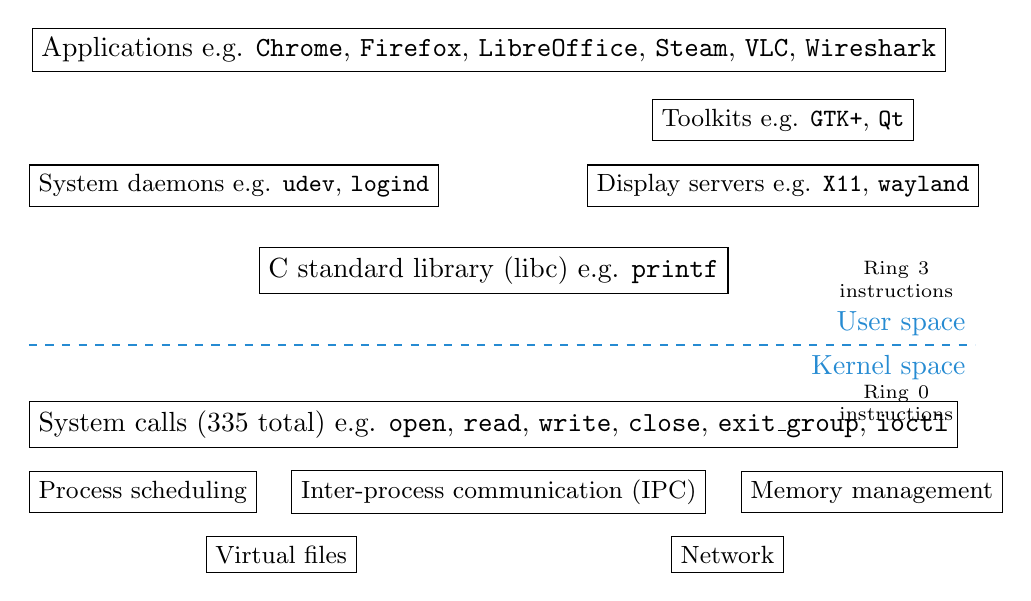
\begin{tikzpicture}[>=stealth']
      \draw [solarizedBlue, dashed, thick] (0,0) -- ($(\textwidth - 3pt, 0)$);
      \node [solarizedBlue, anchor=south east] at ($(\textwidth - 3pt, 0)$)
            (user) {User space};
      \node [solarizedBlue, anchor=north east] at ($(\textwidth - 3pt, 0)$)
            (kernel) {Kernel space};
      \node [anchor=south east, yshift=-0.2em, text width=5em, align=center]
            at (user.north east)
            {\scriptsize Ring 3\\\vspace{-0.5em}instructions};
      \node [anchor=north east, yshift=0.5em, text width=5em, align=center]
            at (kernel.south east)
            {\scriptsize Ring 0\\\vspace{-0.5em}instructions};

      \node [draw, anchor=north west, yshift=-2em] (syscalls) at (0,0)
            {System calls (335 total) e.g. \texttt{open}, \texttt{read},
             \texttt{write}, \texttt{close}, \texttt{exit\_group},
             \texttt{ioctl}};

      \node [draw, below=of syscalls.south west, anchor=north west, yshift=2em]
            (scheduling) {\small Process scheduling};
      \node [draw, right=of scheduling, xshift=-1.6em] (ipc)
            {\small Inter-process communication (IPC)};
      \node [draw, right=of ipc, xshift=-1.6em] (memory)
            {\small Memory management};
      \node [draw, below=of scheduling, yshift=2em, xshift=5em] (virtual)
            {\small Virtual files};
      \node [draw, right=of virtual, xshift=8.5em] (network) {\small Network};

      \node [draw, above=of syscalls, yshift=1em] (libc)
            {C standard library (libc) e.g. \texttt{printf}};
      
      \node [draw, anchor=south west, yshift=-2em] (daemon) at (0, 7em)
            {\small System daemons e.g. \texttt{udev}, \texttt{logind}};
      \node [draw, right=of daemon, xshift=2.5em] (display)
            {\small Display servers e.g. \texttt{X11}, \texttt{wayland}};

      \node [draw, above=of display, yshift=-2em] (toolkit)
            {\small Toolkits e.g. \texttt{GTK+}, \texttt{Qt}};

      \node [draw, above=of daemon.north west, anchor=south west, yshift=0.5em,
             xshift=0.1em] (apps)
            {Applications e.g. \texttt{Chrome}, \texttt{Firefox},
             \texttt{LibreOffice}, \texttt{Steam}, \texttt{VLC},
             \texttt{Wireshark}};
    \end{tikzpicture}
  \end{frame}

  \begin{frame}[fragile]
    \frametitle{System Calls for ``Hello world'' in C, Finding Standard Library}
    \begin{lstlisting}[basicstyle=\ttfamily\footnotesize]
execve("./hello_world_c", ["./hello_world_c"], 0x7ffcb3444f60 /* 46 vars */) = 0
brk(NULL)                               = 0x5636ab9ea000
openat(AT_FDCWD, "/etc/ld.so.cache", O_RDONLY|O_CLOEXEC) = 3
fstat(3, {st_mode=S_IFREG|0644, st_size=149337, ...}) = 0
mmap(NULL, 149337, PROT_READ, MAP_PRIVATE, 3, 0) = 0x7f4d43846000
close(3)                                = 0
openat(AT_FDCWD, "/usr/lib/libc.so.6", O_RDONLY|O_CLOEXEC) = 3
read(3, "\177ELF\2\1\1\3\0\0\0\0\0\0\0\0\3\0>\0\1\0\0\0000C"..., 832) = 832
lseek(3, 792, SEEK_SET)                 = 792
read(3, "\4\0\0\0\24\0\0\0\3\0\0\0GNU\0\201\336\t\36\251c\324"..., 68) = 68
fstat(3, {st_mode=S_IFREG|0755, st_size=2136840, ...}) = 0
mmap(NULL, 8192, PROT_READ|PROT_WRITE, MAP_PRIVATE|MAP_ANONYMOUS, -1, 0)
  = 0x7f4d43844000
lseek(3, 792, SEEK_SET)                 = 792
read(3, "\4\0\0\0\24\0\0\0\3\0\0\0GNU\0\201\336\t\36\251c\324"..., 68) = 68
lseek(3, 864, SEEK_SET)                 = 864
read(3, "\4\0\0\0\20\0\0\0\5\0\0\0GNU\0\2\0\0\300\4\0\0\0\3\0\0", 32) = 32
    \end{lstlisting}
  \end{frame}

  \begin{frame}[fragile]
    \frametitle{System Calls for ``Hello world'' in C, Loading Standard Library}

    \begin{lstlisting}[basicstyle=\ttfamily\footnotesize]
mmap(NULL, 1848896, PROT_READ, MAP_PRIVATE|MAP_DENYWRITE, 3, 0) = 0x7f4d43680000
mprotect(0x7f4d436a2000, 1671168, PROT_NONE) = 0
mmap(0x7f4d436a2000, 1355776, PROT_READ|PROT_EXEC,
  MAP_PRIVATE|MAP_FIXED|MAP_DENYWRITE, 3, 0x22000) = 0x7f4d436a2000
mmap(0x7f4d437ed000, 311296, PROT_READ,
  MAP_PRIVATE|MAP_FIXED|MAP_DENYWRITE, 3, 0x16d000) = 0x7f4d437ed000
mmap(0x7f4d4383a000, 24576, PROT_READ|PROT_WRITE,
  MAP_PRIVATE|MAP_FIXED|MAP_DENYWRITE, 3, 0x1b9000) = 0x7f4d4383a000
mmap(0x7f4d43840000, 13888, PROT_READ|PROT_WRITE,
  MAP_PRIVATE|MAP_FIXED|MAP_ANONYMOUS, -1, 0) = 0x7f4d43840000
close(3)                                = 0
arch_prctl(ARCH_SET_FS, 0x7f4d43845500) = 0
mprotect(0x7f4d4383a000, 16384, PROT_READ) = 0
mprotect(0x5636a9abd000, 4096, PROT_READ) = 0
mprotect(0x7f4d43894000, 4096, PROT_READ) = 0
munmap(0x7f4d43846000, 149337)          = 0
    \end{lstlisting}
  \end{frame}

  \begin{frame}[fragile]
    \frametitle{System Calls for ``Hello world'' in C, Setting Up Heap and
                Printing}

    \begin{lstlisting}[basicstyle=\ttfamily\footnotesize]
fstat(1, {st_mode=S_IFCHR|0620, st_rdev=makedev(0x88, 0x1), ...}) = 0
brk(NULL)                               = 0x5636ab9ea000
brk(0x5636aba0b000)                     = 0x5636aba0b000
write(1, "Hello world\n", 12)           = 12
exit_group(0)                           = ?
+++ exited with 0 +++
    \end{lstlisting}

    \vspace{1em}
    The C version of ``Hello world'' ends with the exact same system calls we
    need
  \end{frame}

  \begin{frame}
    \frametitle{C Calling Convention for x86-64}

    System calls use registers, while C is stack based:
    \begin{itemize}
      \item Arguments pushed on the stack from right-to-left order
      \item \texttt{rax}, \texttt{rcx}, \texttt{rdx} are caller saved
      \item Remaining registers are callee saved
    \end{itemize}

    \vspace{2em}
    What advantages does this give us? Disadvantages?
  \end{frame}

  \begin{frame}
    \frametitle{System Calls are Rare in C}

    Mostly you'll be using functions from the C standard library instead

    \vspace{1em}

    Most system calls have corresponding function calls in C, but may:
    \begin{itemize}
      \item Set \texttt{errno}
      \item Buffer reads and writes (reduce the number of system calls)
      \item Simplify interfaces (function combines two system calls)
      \item Add new features
    \end{itemize}

    \vspace{1em}

    Note: system calls are much more expensive than C function calls (need to
    enter kernel space)
  \end{frame}

  \begin{frame}[fragile]
    \frametitle{System Call vs C Example: \texttt{exit}}

    For an \texttt{exit} (or \texttt{exit\_group}) system call: the program
    stops at that point

    \vspace{1em}

    For \texttt{exit} in C there's a feature to register functions to call
    on program exit: \texttt{atexit}

    \vspace{1em}

    \begin{columns}
      \begin{column}{0.4\textwidth}
        \begin{lstlisting}[basicstyle=\ttfamily\footnotesize]
#include <stdio.h>
#include <stdlib.h>

void fini(void)
{
  puts("Do fini");
}

int main(int argc, char **argv)
{
  atexit(fini);
  puts("Do main");
  return 0;
}
        \end{lstlisting}
      \end{column}
      \begin{column}{0.13\textwidth}
        produces:
      \end{column}
      \begin{column}{0.13\textwidth}
        \texttt{Do main}

        \texttt{Do fini}
      \end{column}
    \end{columns}
  \end{frame}

  \begin{frame}
    \frametitle{Abstraction Example: Memory}

    Operating systems provide \structure{virtual memory}

    \vspace{1em}

    For example if you have 16 GiB of RAM the operating system can use these
    physical addresses: \texttt{0x000000000}---\texttt{0x3FFFFFFFF}

    \vspace{1em}

    As a programmer it seems you have access to all the system's memory

    \vspace{1em}

    The kernel maintains a table of processes mapping virtual addresses to
    physical addresses

    \hspace{1em} Implemented with a hardware translation lookaside buffer (TLB)
                 usually

    \hspace{1em} Often mapped by \structure{pages} (4096 bytes)
  \end{frame}

  \begin{frame}
    \frametitle{What Does Virtual Memory Give Us}

    Ability to run any number of applications, any number of instances

    \hspace{1em} Recall: an executable has a single entry address

    \vspace{2em}

    What's the alternative?

    \begin{itemize}
      \item Each application has to have exclusive access to a region of
            physical memory
      \item Any libraries cannot change size since addresses for libraries need
            to be fixed
    \end{itemize}

    \vspace{2em}

    Other benefits:
    \begin{itemize}
      \item Operating system can map virtual addresses to hardware other than
            physical memory
    \end{itemize}
  \end{frame}

  \begin{frame}
    \frametitle{Normal Compilation in C}

    \begin{center}
    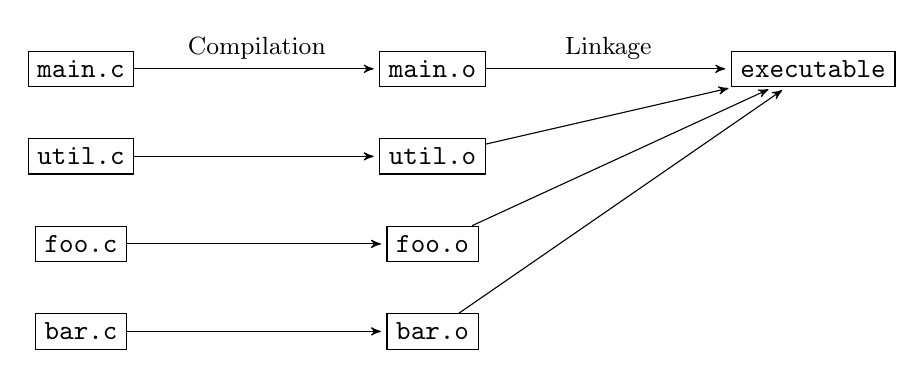
\begin{tikzpicture}[>=stealth', shorten >=2pt]
      \node[draw, align=left] (main) {\texttt{main.c}};
      \node[draw, align=left, below=of main, yshift=1em] (util)
           {\texttt{util.c}};
      \node[draw, align=left, below=of util, yshift=1em] (foo)
           {\texttt{foo.c}};
      \node[draw, align=left, below=of foo, yshift=1em] (bar)
           {\texttt{bar.c}};

      \node[draw, align=left, right=of main, xshift=6em] (main-obj)
           {\texttt{main.o}};
      \node[draw, align=left, below=of main-obj, yshift=1em] (util-obj)
           {\texttt{util.o}};
      \node[draw, align=left, below=of util-obj, yshift=1em] (foo-obj)
           {\texttt{foo.o}};
      \node[draw, align=left, below=of foo-obj, yshift=1em] (bar-obj)
           {\texttt{bar.o}};

      \node[draw, align=left, right=of main-obj, xshift=6em] (exec)
           {\texttt{executable}};

      \draw[->] (main) -- node [above] {\small Compilation} (main-obj);
      \draw[->] (util) -- (util-obj);
      \draw[->] (foo) -- (foo-obj);
      \draw[->] (bar) -- (bar-obj);
      \draw[->] (main-obj) -- node [above] {\small Linkage} (exec);
      \draw[->] (util-obj) -- (exec);
      \draw[->] (foo-obj) -- (exec);
      \draw[->] (bar-obj) -- (exec);
    \end{tikzpicture}
    \end{center}

    \vspace{1em}

    Note: object files (\texttt{.o}) are just ELF files with code for functions
  \end{frame}

  \begin{frame}
    \frametitle{Dynamic Libraries Are For Reusable Code}

    The C standard library is a dynamic library (\texttt{.so}), like any other
    on the system

    \hspace{1em} Basically a collection of \texttt{.o} files containing function
    definitions

    \vspace{1em}

    Multiple applications can use the same library:

    \vspace{1em}

    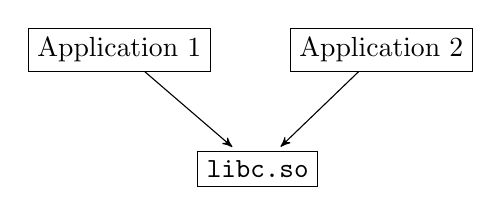
\begin{tikzpicture}[>=stealth', shorten >=2pt]
      \node[draw] (app1) {Application 1};
      \node[draw, right=of app1] (app2) {Application 2};
      \node[draw, below=of app1, xshift=5em] (libc) {\texttt{libc.so}};
      \draw[->] (app1) -- (libc);
      \draw[->] (app2) -- (libc);
    \end{tikzpicture}

    \vspace{1em}

    The operating system only loads \texttt{libc.so} in memory once, and shares
    it

    \hspace{1em} The same physical page corresponds to different virtual pages
    in processes
  \end{frame}

  \begin{frame}
    \frametitle{Useful Command Line Utilities for Dynamic Libraries}

    \texttt{ldd <executable>}

    \hspace{1em} shows which dynamic libraries an executable uses

    \vspace{4em}

    \texttt{objdump -T <library>}

    \hspace{1em} shows the symbols (often just function names) that are in the
    library

    \vspace{1em}

    You can also use \texttt{objdump -d} to disassemble the library
  \end{frame}

  \begin{frame}
    \frametitle{Static vs Dynamic Libraries}

    Another option is to statically link your code

    \hspace{1em} Basically copies the \texttt{.o} files directly into the
    executable

    \vspace{2em}

    The drawbacks compared to dynamic libraries:
    \begin{itemize}
      \item Statically linking prevents re-using libraries, commonly used
            libraries have many duplicates
      \item Any updates to a static library requires the executable to be
            recompiled
    \end{itemize}

    \vspace{2em}

    What are issues with dynamic libraries?
  \end{frame}

  \begin{frame}
    \frametitle{Dynamic Libraries Updates Can Break Executables with ABI
                Changes}

    An update to a dynamic library can easily cause an executable using it to
    crash

    \vspace{1em}

    Consider the following in a dynamic library:

    \hspace{1em} A \texttt{struct} with multiple public fields corresponding to
    a specific data layout (C ABI)

    \vspace{1em}

    \structure{An executable accesses the fields of the \texttt{struct} in the
               dynamic library}

    \vspace{1em}

    Now if the dynamic libraries reorders the fields

    \hspace{1em} The executable uses the old offsets and is now wrong

    \vspace{1em}

    Note: this is OK if the dynamic library never exposes the fields of a
    \texttt{struct}
  \end{frame}

  \begin{frame}[fragile]
    \frametitle{C Uses a Consistent ABI for \texttt{struct}s}

    \texttt{struct}s are laid out in memory with the fields matching the
    declaration order

    \hspace{1em} C compilers ensure the ABI of \texttt{struct}s are the
    consistent for an architecture

    \vspace{2em}

    Consider the following structures:

    \vspace{1em}

    \begin{columns}
      \begin{column}{0.4\textwidth}
        Library v1:
        \begin{lstlisting}[basicstyle=\small\ttfamily]
struct point {
  int y;
  int x;
};
        \end{lstlisting}
      \end{column}
      \begin{column}{0.4\textwidth}
        Library v2:
        \begin{lstlisting}[basicstyle=\small\ttfamily]
struct point {
  int x;
  int y;
};
        \end{lstlisting}
      \end{column}
    \end{columns}

    \vspace{1em}

    For Library v1 the \texttt{x} field is offset by 4 bytes from the start of
    \texttt{struct point}'s base

    \hspace{1em} For Library v2 it is offset by 0 bytes, and this difference
    will cause problems
  \end{frame}

  \begin{frame}[fragile]
    \frametitle{Our Code Should Always Print 3, then 9}

    \begin{lstlisting}[basicstyle=\small\ttfamily]
#include <stdio.h>
#include <stdlib.h>

#include "libpoint.h"

int main(int argc, char **argv)
{
  struct point *p = malloc(sizeof(struct point));
  p->x = 3;
  p->y = 4;
  printf("p.x = %d\n", p->x);
  squareX(p);
  printf("p.x = %d\n", p->x);
  return 0;
}
    \end{lstlisting}

  \end{frame}

  \begin{frame}[fragile]
    \frametitle{Mismatached Versions of This Library Causes Unexpected Results}

    The definition of \texttt{sqaureX} in both libraries is:
    \begin{lstlisting}[basicstyle=\small\ttfamily]
void squareX(struct point *p) {
  p->x *= p->x;
}
    \end{lstlisting}

    \vspace{1em}

    In v1 of the library, this code squares the \texttt{int} at offset 4

    \hspace{1em} v2 squares the \texttt{int} at offset 0

    \vspace{1em}

    If we compile our code against v1, all our \texttt{x}
    accesses are to offset 4 of the \texttt{struct}

    \hspace{1em} Compiling against v2 changes all our \texttt{x} accesses to
    offset 0

    \vspace{2em}
    Compiling against a version of the library and using another
    causes unexpected results:

    \hspace{1em} It will always print 3 followed by 3

    \hspace{2em} Matching the versions prints 3 followed 9, as expected
  \end{frame}

  \begin{frame}[fragile]
    \frametitle{Try the Previous Example}

    It uses the \texttt{LD\_LIBRARY\_PATH} trick (mentioned again later) to
    simulate a library update

    \vspace{2em}

    Run the following commands to see for yourself:
    \begin{lstlisting}[commentstyle={}]
git clone https://github.com/eyolfson/talks
cd talks/2019/ucla-cs-111-lecture-2
make
make run_my_code_compiled_with_point_v1_with_point_v1
make run_my_code_compiled_with_point_v2_with_point_v1
make run_my_code_compiled_with_point_v1_with_point_v2
make run_my_code_compiled_with_point_v2_with_point_v2
    \end{lstlisting}
  \end{frame}

  \begin{frame}
    \frametitle{Semantic Versioning Meets Developer's Expectations}

    From \url{https://semver.org/}, given a version number MAJOR.MINOR.PATCH,
    increment the:

    \begin{itemize}
      \item MAJOR version when you make incompatible API\structure{/ABI} changes
      \item MINOR version when you add functionality in a backwards-compatible
            manner
      \item PATCH version when you make backwards-compatible bug fixes
    \end{itemize}
  \end{frame}

  \begin{frame}[fragile]
    \frametitle{Dynamic Libraries Allow Easier Debugging}

    Control dynamic linking with environment variables (e.g.
    \texttt{LD\_LIBRARY\_PATH} and \texttt{LD\_PRELOAD})

    \vspace{2em}

    Consider the following example:
    \begin{lstlisting}[basicstyle=\small\ttfamily]
#include <stdlib.h>
#include <stdio.h>

int main(int argc, char **argv)
{
  int *x = malloc(sizeof(int));
  printf("x = %p\n", x);
  free(x);
  return 0;
}
    \end{lstlisting}
  \end{frame}

  \begin{frame}[fragile]
    \frametitle{We Can Monitor All Allocations with Our Own Library}

    Normal runs of \texttt{alloc\_test} outputs:
    \begin{lstlisting}[basicstyle=\small\ttfamily]
x = 0x561116384260
    \end{lstlisting}

    \vspace{1em}

    Create \texttt{myalloc.so} that outputs all \texttt{malloc} and
    \texttt{free} calls

    \vspace{1em}

    Now we run with \texttt{LD\_PRELOAD=./myalloc.so  ./alloc\_test} which
    outputs:
    \begin{lstlisting}[basicstyle=\small\ttfamily]
Call to malloc(4) = 0x55c12aa40260                  
Call to malloc(1024) = 0x55c12aa40280
x = 0x55c12aa40260
Call to free(0x55c12aa40260)
    \end{lstlisting}

    \vspace{1em}

    Interesting, we did not make 2 \texttt{malloc} calls
  \end{frame}

  \begin{frame}
    \frametitle{Detecting Memory Leaks}

    \texttt{valgrind} is another useful tool to detect memory leaks from
    \texttt{malloc} and \texttt{free}

    \hspace{1em} Usage: \texttt{valgrind <executable>}

    \vspace{1em}

    Here's a note from the \texttt{man} pages regarding what we saw:

    \textit{The GNU C library (\texttt{libc.so}), which is used by all programs,
      may allocate memory for its own uses. Usually it doesn't bother to free
      that memory when the program ends—there would be no point, since the Linux
      kernel reclaims all process resources when a process exits anyway, so it
      would just slow things down.}

    \vspace{1em}

    \structure{Note: this does not excuse you from not calling \texttt{free}!}
  \end{frame}

  \begin{frame}
    \frametitle{Abstraction Example: File Descriptors}

    File descriptors are just a number and may used to represent:
    \begin{itemize}
      \item Regular files
      \item Directories
      \item Block devices
      \item Character devices
      \item Sockets
      \item Named pipes
    \end{itemize}

    All of these can be used with \texttt{read} and \texttt{write} system calls

    \vspace{1em}

    Kernel maintains a per-process file descriptor table
  \end{frame}

  \begin{frame}
    \frametitle{Standard File Descriptors for Unix}

    All command line executables use the following standard for file
    descriptors:

    \begin{itemize}
      \item \texttt{0} --- \texttt{stdin} (Standard input)
      \item \texttt{1} --- \texttt{stdout} (Standard output)
      \item \texttt{2} --- \texttt{stderr} (Standard error)
    \end{itemize}

    \vspace{2em}

    The terminal emulators job is to:
    \begin{itemize}
      \item Translate key presses to bytes and write to \texttt{stdin}
      \item Display bytes read from \texttt{stdout} and \texttt{stderr}
      \item May redirect file descriptors between processes
    \end{itemize}
  \end{frame}

  \begin{frame}[fragile]
    \frametitle{Checking Open File Descriptors on Linux}

    \texttt{/proc/<PID>/fd} \hspace{0.5em} is a directory containing all open
    file descriptors for a process

    \texttt{ps x} \hspace{0.5em} command shows a list of processes matching your
    user (lots of other flags)

    \vspace{1em}

    A terminal emulator may give the output:
    \begin{lstlisting}[basicstyle=\small\ttfamily]
> ls -l /proc/21151/fd
0 -> /dev/tty1
1 -> /dev/tty1
2 -> /dev/tty1
    \end{lstlisting}

    \vspace{2em}

    \texttt{lsof <file>} \hspace{0.5em} shows you what processes have the file
    open

    \hspace{2em} For example, processes using C: \hspace{0.5em}
    \texttt{lsof /lib/libc.so.6}
  \end{frame}

  \begin{frame}
    \frametitle{Lessons Learned Today}

    \begin{itemize}
      \item Basic executable format (ELF files)
      \vspace{1em}
      \item Difference between API and ABI
      \vspace{1em}
      \item How to find all system calls
      \vspace{1em}
      \item Virtual memory and why it's needed
      \vspace{1em}
      \item Dynamic libraries and a comparison to static libraries
      \vspace{1em}
      \item File descriptors and standard conventions
    \end{itemize}
  \end{frame}
\end{document}
